%
%\documentclass[useAMS,8pt,twocolumn]{article}
\documentclass[apj]{emulateapj}
\bibliographystyle{apj}

%\pdfpagewidth  200mm
%\pdfpageheight 297mm
%\addtolength{\oddsidemargin}{-.4in}
%%\addtolength{\evensidemargin}{-.4in}                                           
%\addtolength{\textwidth}{1.1in}
%\addtolength{\topmargin}{-.5in}
%\addtolength{\textheight}{1.6in}


%\usepackage[T1]{fontenc}
%\usepackage[latin9]{inputenc}
%\usepackage{geometry}
%\geometry{verbose,letterpaper,tmargin=2cm,bmargin=2cm,lmargin=2cm,rmargin=2cm}
\usepackage{apjfonts}
\usepackage{graphicx}
\usepackage{color}
\usepackage{amsbsy}
%\usepackage{mathrsfs}
\usepackage{mathpazo,bm}
\usepackage{amsmath}
\usepackage{multirow}
\usepackage{natbib}
\usepackage{amssymb}


\newlength{\hfwidth}
\newlength{\hfwidthsingle}
\addtolength{\hfwidthsingle}{.5\textwidth} %single fig in figure
\addtolength{\hfwidth}{.497\textwidth} %single fig in figure*

\newcommand{\pderiv}[2]{\frac{\partial #1}{\partial #2}}
\newcommand{\pderivn}[3]{\frac{\partial^{#3} #1}{\partial #2^{#3}}}
\newcommand{\vt}[1]{\mathbf{#1}}       %for tensors
\renewcommand{\v}[1]{{\boldsymbol{#1}}} %for vectors
\newcommand{\Ro}{\mathrm{Ro}}
\def\white#1{\textcolor{white}{#1}}
\definecolor{brown}{rgb}{0.42,0.24,0.07}
\def\brown#1{\textcolor{brown}{#1}}
\newcommand{\comm}[1]{({\it \brown{#1}})}
\newcommand{\del}{\v{\nabla}}
\newcommand{\grad}{\del}
\newcommand{\Div}{\del\cdot}
\newcommand{\Divp}[1]{\del\cdot\left(#1\right)}
\newcommand{\curl}{\del\times}
\newcommand{\Laplace}{\nabla^2}
\newcommand{\de}{\mathrm{d}} 
\newcommand{\rint}{$s_{\rm int}\,$}
\newcommand{\rext}{$s_{\rm ext}\,$}
\newcommand{\hats}{\hat{\v{s}}}
\newcommand{\hatphi}{\hat{\v{\phi}}}
\newcommand{\hatz}{\hat{\v{z}}}
\newcommand{\hatx}{\hat{\v{x}}}
\newcommand{\haty}{\hat{\v{y}}}
\newcommand{\hatm}{{\hat{m}}}
\newcommand{\hatn}{{\hat{n}}}
\newcommand{\he}{{\hat{e}}}
\newcommand{\hmu}{{\hat{\mu}}}
\newcommand{\hnu}{{\hat{\nu}}}
\newcommand{\va}{v_{_{\rm A}}}
\newcommand{\eps}{\epsilon}
\newcommand{\cte}{\textrm{cte}}
\newcommand{\up}{u^\prime}
\newcommand{\pp}{p^\prime}

\newcommand{\Eq}[1]{Eq. (\ref{#1})}
\newcommand{\Eqs}[2]{Eqs. (\ref{#1}) and~(\ref{#2})}
\newcommand{\Eqss}[2]{Eqs. (\ref{#1})--(\ref{#2})}
\newcommand{\eq}[1]{\Eq{#1}}
\newcommand{\eqs}[2]{\Eqs{#1}{#2}}
\newcommand{\eqss}[2]{\Eqss{#1}{#2}}
\newcommand{\eqp}[1]{(Eq. \ref{#1})}

\newcommand{\App}[1]{Appendix~\ref{#1}}
\newcommand{\app}[1]{\App{#1}}
\newcommand{\Figure}[1]{Figure~\ref{#1}}
\newcommand{\Fig}[1]{Fig.~\ref{#1}}
\newcommand{\fig}[1]{\Fig{#1}}
\newcommand{\Figs}[2]{Figs.~\ref{#1} and \ref{#2}}

\newcommand{\beq}{\begin{equation}}
\newcommand{\eeq}{\end{equation}}
\newcommand{\beqn}{\begin{eqnarray}}
\newcommand{\eeqn}{\end{eqnarray}}
\newcommand{\epsp}{\varepsilon_{_{+}}}
\newcommand{\epsm}{\varepsilon_{_{-}}}

\shorttitle{Dust in disk vortices}
\shortauthors{Lyra \& Lin}

\slugcomment{Draft version}

\begin{document}
%\date{}

\title{Steady state of dust distributions in disk vortices}
\author{Wladimir Lyra\altaffilmark{1,2,3,$\star$} and Min-Kai Lin\altaffilmark{4,$\star$}}
\email{wlyra@caltech.edu, \ mklin924@cita.utoronto.ca}
\altaffiltext{1}{Jet Propulsion Laboratory, California Institute of Technology, 4800 Oak Grove Drive, Pasadena, CA, 91109, USA}
\altaffiltext{2}{Division of Geological \& Planetary Sciences, California Institute of Technology, 1200 E California Blvd MC 150-21, Pasadena, CA 91125 USA}
\altaffiltext{3}{Sagan Fellow}
\altaffiltext{4}{Canadian Institute for Theoretical Astrophysics , 60
  St. George Street, Toronto, Ontario, M5S 3H8, Canada}
\altaffiltext{$\star$}{Both authors contributed equally to this work}

\begin{abstract}
.
\end{abstract}

\section{Introduction}
\label{sect:introduction}

% These changes are: small near-IR excesses, significant mid and far-IR
%excesses. (near-IR -> 1-5mu, mid-IR -> 5-20 mu, far-IR beyond 20 mu) 

% mid excess => wall
% far IR => Cold dust
% near IR => some (pre-transitional), evidence of optically thick warm dust, small inner disk 

Transitional disks are a class of disks that lacks a near infrared
excess, implying absense of optically thick warm dust in the inner
disk. At the same time, these disks show signatures of cold gas in the
outer disk, and 50\% of such disks show signs of accretion (Calvet et
al. 2005, Espaillat et al. 2007, \comm{check, quote relevant works}). 
The age of these disks, in the 1-10 Myr range, suggests that they are undergoing 
the evolutionary stage between gas-rich protoplanetary disks and gas-poor
debris disks. The absense of dust in the inner disk is usually
attributed to the planet formation process, supposed to be completed
or nearly completed in that region. 

% classic T-Tauri star (CTTS, full continuous IR excess from NIR to
% mm), to WTTS with bare stellar photospheres. 

%Transition disks have been defined as objects with no detectable
%near-IR excess, steep slopes in the mid-IR, and large far-IR excesses
%(e.g., Muzerolle et al. 2006; Sicilia-Aguilar et al. 2006b). Relaxed
%(Brown et al. 2007; Cieza et al. 2008) 
%to include some NIR excess. Pre-transitional (Espaillat et al. 2008,
%disks with thick inner dust, optically thin gas, and thick outer
%dust). 

%Disk evolution processes include viscous accretion (Hartmann et al. 1998), photoevaporation (Alexander et al. 2006), the mag- netorotational instability (Chiang & Murray-Clay 2007), grain growth and dust settling (Dominik & Dullemond 2008), planet formation (Lissauer 1993; Boss 2000), and dynamical inter- actions between the disk and stellar or substellar companions (Artymowicz & Lubow 1994).

%giant planet formation, grain growth (Dominki & Dullemond),
%photoevaporation (Owen), and tidal
%truncation in close binaries (Artymowicz, Ireland & Kraus 08).
%CoKu Tau/4 has been shown to be a close binary star system with an 8
%AU projected separation, rendering its disk a circumbinary one
%(Ireland & Kraus 2008).
%(Quillen et al. 2004: planet), but Najita et al. (2007: photoevaporation) 

%Individual disks: TW Hydra (Calvet et al. 2004), GM Aur and DM Tau (Calvet et al. 2005), LkHα 330 (Brown et al. 2008), and LkCa 15 (Espaillat et al. 2008).
%groups: Najita et al 07: most disks consistent with planet formation
%scenario; Cieza et al. 08, strong constrast, finding photoevaporation
%to be dominant. Cieza et al. 10 -> 9/26 photo, 13/26 grain growth,
%4/26 binaries, 4/26 planets. 

%Strom et al. 1989 : identification (opacity hole) 
%others on identification: Skrutskie et al. 1990 (suggested gap model)
%others on identification: Gauvin & Strom 1992; Marsh & Mahoney 1992; Wolk & Walter 1996
%Calvet et al. 2005 : coined term
%Espaillat et al. 2007 : census
%Najita et al 2007 : census
%Espaillat et al. 2008: confirmation of gap in LkCa 15
%Cieza et al. 2008 :inner disks start to dissipate only after the outer disk has been significantly depleted of mass. This provides
%                                      strong support for
%                                      photoevaporation
%Evans et al. 2009: nomenclature
%Cieza et al. 2010: heterogeneous; grain growth, planet gaps, photoevaporation, stellar companions.
%Espaillat et al. 2010: refined the gap model of 2008, includes shadows and all sorts of sophistications, extends to other disks. 
%Kim et al. 2009: just a work
%Merin et al. 2010: census, favor planet formation, only 25% show no accretion, making it unlikely that photoevaporation 
%                             is the dominant hole-forming process in most cases. 
%Muzerolle et al. 2010: census, 
%It must be noted that - Clarke & Owen, not clear if transitional disks are associated with planets at all. 

%Espaillat et al. 2012: nomenclature
%Evans 09: The Diskionary: A Glossary of Terms Commonly Used for Disks and Related Objects, First Edition

% transition disks: young stars with spectral evidence for cool 
% dust but which lack diagnostic of warm dust
%
% colder: big hole; warmer: small hole
% 

% Hughes et al. 2007 2009, Andrews et al. 2009, 2010, 2011, for 
% confirmed with sub-mm and mm interferometric imaging that TDs have
% truncated outer edges. Thalmann et al. 2010 does the same for LkCa 15
% for NIR imaging. 

%Optically thick inner disk of PTD : veiling of NIR (Espaillat et al. 2008a, 2010)

%NIR interferometry confirms that the inner disk is small (Pott et al. 2010, 
% Olofsson et al. 2011) 

% potential planets claimed: Kraus et al. 2011 (LkCa 15), Huelamo et al. 2011
% (T Cha). 

%Disks undergoing clearing: Lada et al. 2006, Hernandez et al. 2007,
%Cieza et al. 2010, Muzerolle et al. 2010, Luhman et al. 2010, Merin et al. 
%2010, Currie & Sicilia-Aguilar 2011. 

% 



Since the early images of transitional disks, a variety of deviations
from axisymmetry have been observed in the outer disk \comm{quote works}. These asymmetries 
have recently been observed with the Atacama Large Millimeter Array
(ALMA), showing large lopsided dust distributions \comm{quote works}. The explanation in
vogue borrows from the protoplanetary disk literature by suggesting that these asymmetries are the
result of dust trapping in giant anticyclonic vortices. 

Trapping of solids in gas vortices was independently suggested
by Barge \& Sommeria (1995) and Tanga et al. (1996) as a route for
planet formation in the inner regions of circumstellar
disks. Particles trapping in a vortex is analog to the particle drift
that happens in the disk
itself. The gas in the disk rotates at a slight sub-Keplerian rate,
because the pressure, decreasing outwards, opposes gravity,
lowering the amount of angular momentum needed to achieve centrifugal
equilibrium. A particle does not feel the pressure gradient, orbiting at
the Keplerian velocity in the absense of drag forces. The particle
thus travels faster than the gas, feeling a
headwind and sinking. In a vortex, gravity is substituted by the
Coriolis force, leading to a similar result. Particles experience a
drag force, lose angular momentum, and sink toward the vortex
center, where they accumulate. Klahr \& Henning (1997) applied the model 
to turbulent eddies in the solar nebula, finding trapping of mm-sized
particles preferentially \comm{why this wrong result?}, and suggested
this could aid on the formation of chondrules. The dynamics of dust
trapping in vortices was developed by Chavanis (2000), a detailed work 
that set the analytical foundations of the field \comm{model,
  limitations, results?}.  

The first attempt to simulate the process with
fully nonlinear compressible hydrodynamics was carried by Johansen et
al. (2004), imposing a vortex solution into a  shearing box (a Cartesian box sampling a small
patch of the disk, co-rotating with the flow at a fixed distance from
the star, see e.g. Hawley et al. 1995, Umurhan 2010). The model had limitations, chiefly the use of Laplacian
viscosity, that limited the lifetime of the vortex, and the symmetries
imposed by the shearing box, that affected the geometry and evolution
of the vortex.  Both effects combined did not allow the
imposed vortex solution to survive for more than a single orbit, but
nonetheless the vortex ability to trap dust was validated. 

These studies, however, did not consider the question of how to
form disk vortices in first place. Because vortices are exact nonlinear solutions to the equations of
hydrodynamics, these works used analytical vortex solutions, and remained
agnostic with respect to their origin. As it turns out, forming and
sustaining disk vortices proved to be a formidable problem in
itself. Because of the strong stabilizing effect of the Keplerian
shear, formation mechanisms rely on modifications of the shear
profile, in what have been called ``edge modes''. These modes have
first been found by Hohfeld \& Lovelace (1978), and mentioned en
passant by Toomre (1981), both in the context of galactic disks. The first detailed analysis of their
(in)stability properties was provided by Papaloizou \& Pringle (1985) in the
context of ``thick tori'' accretion disks around
black holes, a work that was followed by Hawley et al. (1987), that
simulated the process, and showed that the instability saturates into
vortices. It was the hope back then that this process, that became
known as ``Papaloizou-Pringle instability'', would generate the
long-sough mechanism for accretion, but the fact that it needed a
modification of the shear profile did not play into its favor. 

Though the interest on this process waned rapidly after the re-discovery of the MRI
(Velikhov 1959, Chandrasekhar 1961) by Balbus \& Hawley (1991), and
its rise to paradigmatic status as the main source of angular momentum
transport in accretion disks, it is still valid for forming
vortices. The calculation was brough to the context of cold disks by
Lovelace et al. (1999), who also extended the analysis to
non-barotropic disks, and renamed the process Rossby wave instability
(RWI), due to a similarity between the unstable modes and the
meandering waves in planetary weather. While in the context of thick
tori models the modification of the shear profile may not come about
easily, the situation is different in protoplanetary
disks. Simulations show that two processes naturally form such
profiles. One is the boundary between the MRI-active magnetized zone
and the MRI-dead resistive zone; in the transition, a resistivity
inversion occurs, with matter piling up, generating the favourable
shear profile (Varni\`ere et al. 2006). The accumulation of dust in RWI vortices at dead zone boundaries was
studied at first by Inaba \& Barge (2006), who found that \comm{what
  did they find?}. The other is at the edge of a
gap opened by a planet. That the gap edge is unstable to the RWI is seen in
the inviscid simulations of many codes in the code comparison study of
de Val-Borro et al. (2006). The process was studied in detail by de
Val-Borro et al. (2007). 

These efforts culminated into a coherent picture of vortex-assisted
planet formation in dead zone vortices by Lyra et al. (2008, 2009a) and in 
gap edge vortices by Lyra et al. (2009b). These works solved
selfconsistently for the nonlinear compressible hydrodynamics and the
aerodynamics of interacting solid particles, in inviscid models in the
inertial frame, removing the limitations in Johansen et al. (2004),
albeit in the context of 2D disks. These works inspired a renewed
interest in the RWI, that has been vigorously studied in three
dimensions by Meheut et al. (2010, 2012a, 2012b, 2012c) , Lin \&
Papaloizou (2011),  Lin (2012, 2013ab), and Lyra \& Mac Low (2012)
\comm{tell what these studies found}. 

Part of these results have been translated to the field of
transitional disks. The main difference is that while the focus 
of vortex dust-trapping research in protoplanetary disks is the
concentration of pebbles rocks and boulders in the inner disk to form
planets, in transitional disks the focus is on the trapping of sub-mm
and mm-size dust in the outer disk to match the observed lopsided 
asymmetries. While the motivation and dust sizes are different, the
physics is scale-free and almost identical. The particle size that is
preferentially trapped is set by the friction time, $\tau_{\rm f}$, which is a
function of the gas density and particle radius. A suitable nondimensionalization for the
friction time is the Stokes number, St = $\varOmega \tau_{\rm f}$,
where $\varOmega$ is the Keplerian frequency. While in the dense, fast
rotating, inner regions of T-Tauri disks, the best particle size (St =1, e.g. 
Youdin \& Goodman 2005, Youdin 2008)
corresponds to meter-size, in the thin, outer regions of transitional
disks, the size corresponding to St=1 drops by about three orders of
magnitude. The resulting trapping of sub-mm and mm-size dust may not
lead to the critical densities necessary to form planets, but they may
well explain the puzzling observed lopsided asymmetries. 

Reg\'aly et al. (2012) suggested that the sub-mm 
observations of Brown et al. (2009) could be the result of dust
trapping in vortices that, they suggest, could be triggered at dead
zone edges, as in Varni\`ere et al. (2006), Inaba \& Barge (2006), and Lyra et
al. (2008, 2009a). The dead zone mechanism is probably not reasonable,
because the radii is quite far out, and the outer edge of the dead
edge is quite smooth (Dzyuerkevich 2010, Neal 2013). It is probably
not the result of baroclinic instability either, because the outer
disk is isothermal, and the baroclinic instability requires a negative
entropy gradient. This leaves gap-edge RWI as a plausible mechanism. 

If indeed the asymmetries are due to gap edge Rossby vortices, then, 
as the drag force drives dust toward the vortex center, diffusion is
needed to maintain a steady state over the lifetime of the disk. 
%\footnote{{This
%diffusion is the result of elliptic instability and in general
%different than the diffusion in the gas phase (see e.g., Lyra \& Klahr
%2011)}}. 
Steady state solutions should exist in this case and, indeed, Ataiee
et al. (2013), modeling particles of different Stokes numbers, finds
two different dust distributions, as expected. Birnstiel et al. (2013) 
presented a semi-analytical model that solves for the azimuthal dust 
distribution while using fits from numerical simulations (Pinilla et al. 2012)
to constrain the radial morphology. In this work we present an analytical 
model for the steady state distribution of dust trapped in vortices, 
accurate to first order in Stokes number, and general in space. In 
Section 2 we derive the
advective-diffusive equation, and in Sect 3 the appropriate coordinate
transformation. In Sect 4 we solve the equation for the axisymmetric
case, and in Sect 5 we generalize it for non-axisymmetry. Concluding
remarks follow. 


%that yields the dust density
%distribution. The solution, however, makes use of the stringent
%approximation of canceling the radial pressure gradient, so it applies
%only at the radial location of a pressure maximum; it effectively
%describes an infinitesimally narrow ring.  



%Due to the drag force, dust trapped in vortices will accumulate in the
%center. Diffusion is needed to maintain a steady state over the
%lifetime of the disk. In here, we seek to obtain steady state solution
%of the diffusion-advection equation of dust in the possible vortices 
%seen in the observations. 




%Outline of the Introduction: 
%- Definition of transitional disks
%- Asymmetries in these disks (signposts of planets)
%- BORROWS from the planet formation and protoplanetary disk literature
%to suggest vortices
%- RWI is a well studied process
%- Dust trapping: mention works of: 
%Barge & Sommeria; 
%Tanga et al. (initial ideas) ;
%Klahr & Henning 1997
%Chavanis 2000 - detailed study of dust trapping, 
%Anders' article 2004, used that to simulate dust trapping in a
%shearing sheet; agnostic about vortex formation mechanism;
%(check Fred Adams, see if there's anything in there)
%Papa & Pringle 84, Hawley 87 ; Lovelace et al. 99, Li et al. 00 (RWI)
%Varniere & Tagger 06, dead zones
%de Val Borro et al. 2006 (many codes); 2007 vortex trapping by itself
%culminated in the planet-forming model assisted by vortex trapping in
%dead zone vortices (Lyra et al. 2008, 2009a) and gap edge vortices
%(Lyra et al. 09b). 
%A renaissance was sparkled in the study of the RWI, e.g., Min-Kai's
%and Heloise's work.  
%(mention other methods for producing vortices, and why they fail for
%transitional disk - dead zone to far out, baroclinic can't go in isothermal)

%Recently transitional disks have become a new venue for exploring the
%physics of vortex trapping. 

%Works on dust with ALMA: Cassasus, Isela, Nienke
%* Wilner et al. 2002 - 3Mj at 40 AU with e=0.6 (check how's that now) 

%ALMA is returning images of transitional disks in which large
%asymmetries are seen in the dust distribution of mm-size in the outer
%disk. The explanation in vogue borrows from the protoplanetary disk 
%literature by suggesting that these asymmetries are the
%result of dust trapping in giant vortices. The vortex excitation method would
%be Rossby Wave Instability (RWI) at planetary gap edges. 


\section{Dust steady state} 
\label{sect:model-equations}

Considering the dust is of small sizes, we can treat it as a
fluid. The dust should then follow the continuity equation 

\beq
  \pderiv{\rho_d}{t} = -(\v{v}\cdot\del)\rho_d - \rho_d \Div{\v{v}} + D\Laplace{\rho_d},
  \label{eq:continuity}
\eeq

\noindent where $\rho_d$ is the dust density, $\v{v}$ is the dust
velocity, and $D$ is the diffusion coefficient (the diffusion is due
to elliptical turbulence in the vortex core and in general will be
different than the turbulent viscosity in the disk). We assume $D$ is
constant. 

To derive the velocities, instead of solving the momentum equations
for the dust, we make use of the relative velocity, following Youdin \& Goodman (2005,
see also Youdin 2008)  

\beq
\v{v} = \v{u} + \tau  \grad{h}, 
\label{eq:v}
\eeq

\noindent where $\v{u}$ is the gas velocity. Equation~\ref{eq:v} is 
accurate to first order in friction time $\tau$, assumed 
constant. The enthalpy $h$ is defined as $dh = dp /\rho$, where $p$ 
is the pressure and $\rho$ the gas density. 

Inside the vortex, the flow is divergenceless, and 
we adopt the following model for $\v{u}$
\beq
  u_x = \varOmega_V y / \chi \qquad  u_y= -\varOmega_V x \chi
  \label{eq:vortex}
\eeq
\noindent for a vortex of aspect ratio $\chi= y/x > 1$. The Kida
solution $\varOmega_V = 3\Omega_K/2(\chi-1)$ smoothly matches 
this velocity field to the Keplerian shear. We note that the dust
velocity is comprised of a divergence-free part, $\v{u}$, and a
curl-free part, $\tau\grad{h}$. The vortex flow attempts to keep the
dust particles on closed elliptic streamlines, via $\v{u}$, while friction
attempts to concentrate dust toward pressure maximum, via $\tau\grad
h$. The only effect that attempts to spread out the dust is diffusion, via $D$.  

Taking the divergence of
\eq{eq:v} gives 

\beq
\Div{\v{v}} = \tau \Laplace{h}, 
\label{eq:divv}
\eeq

\noindent and we can find the Laplacian of the enthalpy via the Euler
equation. Adopting the shearing sheet approximation, in steady state
the force balance yields  

\begin{eqnarray}
\pderiv{h}{x} &=& 3\varOmega^2 x + 2\varOmega u_y -
u_y\pderiv{u_x}{y} \nonumber \\
&=& \left(3\varOmega^2 - 2\Omega\Omega_V \chi + \varOmega_V^2\right) x
= -\frac{C_1}{\tau} \  x,  \\
\pderiv{h}{y} &=& - 2\varOmega u_x -
u_x\pderiv{u_y}{x} \nonumber \\
&=& \left(-2\Omega\Omega_V/\chi + \Omega_V^2\right) y = -\frac{C_2}{\tau} \  y.
\end{eqnarray}

\noindent  Substituting the equations above into \eq{eq:divv}, also
with $\omega_{_V}=\varOmega_V/\varOmega$, the divergence becomes 

\beqn
\Div{\v{v}} &=& -(C_1+C_2) = - C \label{eq:const-div}\\
&=& - \tau\varOmega^2
\left[2\omega_{_V}\left(\frac{\chi^2+1}{\chi}\right) - (2\omega_{_V}^2
  + 3) \right], 
\label{eq:scale-div}
\eeqn

\noindent where we define $C$ as positive, so that the divergence is negative (physically meaning that the dust gets trapped). Replacing \eq{eq:const-div} in the continuity equation, and setting $\partial_t$ =
0 for steady state, 

\beq
\left(D\Laplace{} -  \v{v}\cdot\del  + C\right)\rho_d = 0. 
\label{eq:steady}
\eeq

Substituting the gas velocity, and dividing by $D$, we
arrive at the modified advection-diffusion equation that should
determine the steady-state distribution of the vortex-trapped dust, 

%\beq
%   -\Omega_V y / \chi \partial_x \rho_d +  \Omega_V x \chi \partial_y
%  \rho_d + C \rho_d  + D\partial_x^2{\rho_d} + D\partial_y^2{\rho_d} = 0.
%\eeq

%Dividing by $D$ and substituting $A=\varOmega_V/D$ and $B=C/D$, we
%arrive at the modified advection-diffusion equation that should
%determine the steady-state distribution of the vortex-trapped dust.

%\beqn
%&&  \pderivn{\rho_d}{x}{2} + \pderivn{\rho_d}{y}{2} - \left(Ay\chi^{-1} - B_1x\right) \pderiv{\rho_d}{x} +\\  
%&& \quad \left(A x \chi + B_2y\right) \pderiv{\rho_d}{y} + B \rho_d   = 0 
%\eeqn

\beq
\left[\Laplace{} - \left(Ay\chi^{-1} - B_1x\right) \partial_x  +
  \left(A x \chi + B_2y\right) \partial_y + B \right] \rho_d   = 0,  
\label{eq:dust-trapping-cartesian}
\eeq
\\
\noindent where we also substituted  $A=\varOmega_V/D$ and $B_i=C_i/D$.

\section{Change of variable}

We change variables to the coordinate system used in Chang \& Oishi (2010)

\beqn
  x &=& a \cos\nu, \label{eq:change-x}\\
  y &=& a\chi\sin\nu.  \label{eq:change-y}
\eeqn

The system is not orthogonal, but it has the advantage of matching the
aspect ratio of the ellipses (In contrast, the elliptic coordinate
system, though orthogonal, describes a system of confocal ellipses of
different aspect ratio, that does not coincide with the geometry of
the problem). In these coordinates, the transformations are 

%$\partial_\v{a} =
%\vt{A} \partial_\v{x}$, and $\partial_\v{x} =
%\vt{A}^{-1} \partial_\v{a}$, with $\v{a} = (a,\nu)^T$, and $\v{x} =
%(x,y)^T$. That is

\beq
\left[\begin{array}{c}
    \partial_{a}  \\
    \partial_{\nu}
  \end{array}\right] = \vt{A} 
  \left[\begin{array}{c}
      \partial_{x}  \\
      \partial_{y}
    \end{array}\right] 
%
\quad {\rm and} \quad 
%
\left[\begin{array}{c}
    \partial_{x}  \\
    \partial_{y}
  \end{array}\right] = \vt{A}^{-1} 
  \left[\begin{array}{c}
      \partial_{a}  \\
      \partial_{\nu}
    \end{array}\right],  
%
\eeq

\noindent with 

\beq
\vt{A} = \left[\begin{array}{cc}
\pderiv{x}{a}  & \pderiv{y}{a}  \\
\pderiv{x}{\nu}  & \pderiv{y}{\nu} \\
\end{array}\right] = \left[\begin{array}{cc}
\cos\nu  & \chi\sin\nu  \\
-a\sin\nu  & a\chi\cos\nu \\
\end{array}\right]. 
\eeq

\noindent The inverse matrix is 

\beq
\vt{A}^{-1} = \frac{1}{a\chi} \left[\begin{array}{cc}
a\chi\cos\nu  & -\chi\sin\nu  \\
a\sin\nu  & \cos\nu \\
\end{array}\right].  
\eeq

The transformations are therefore

\beqn
\pderiv{}{x} &=& \cos\nu \pderiv{}{a} - \frac{\sin\nu}{a} \pderiv{}{\nu}, \\
\pderiv{}{y} &=& \frac{1}{\chi}\left(\sin\nu \pderiv{}{a} + \frac{\cos\nu}{a} \pderiv{}{\nu} \right),
\eeqn

%And the second derivatives are 

%\beqn
%\pderivn{}{x}{2} &=& \left(\cos\nu \pderiv{}{a} - \frac{\sin\nu}{a}
%  \pderiv{}{\nu}\right) \left(\cos\nu \pderiv{}{a} -
%  \frac{\sin\nu}{a} \pderiv{}{\nu}\right) \nonumber \\ \\
%&=& \cos^2\nu\partial^2_a + a^{-2}\sin^2\nu \partial^2_\nu -
%a^{-1}\sin 2\nu \partial^2_{a\nu} \nonumber \\
%&&+ a^{-2}\sin 2\nu\partial_\nu +
%a^{-1}\sin^2\nu \partial_a 
%\eeqn

%\beqn
%\pderivn{}{y}{2} &=& \frac{1}{\chi^2}\left(\sin\nu \pderiv{}{a} +
%  \frac{\cos\nu}{a} \pderiv{}{\nu} \right) \left(\sin\nu
% \pderiv{}{a} + \frac{\cos\nu}{a} \pderiv{}{\nu} \right) \nonumber
%\\ \\
%&=& \frac{1}{\chi^2}\left[ \sin^2\nu \partial^2_a +
%  a^{-2}\cos^2\nu \partial^2_\nu + a^{-1}\sin
%  2\nu \partial^2_{a\nu}\right. \nonumber \\
%&&\left.- a^{-2}\sin 2\nu \partial_\nu +
%  a^{-1}\cos^2\nu \partial_a \right] 
%\eeqn

\noindent and the Laplacian is thus 

\beqn
\Laplace{} &= &\frac{1}{2}\left[ \epsm \cos 2\nu +  \epsp\right] \partial^2_a  \nonumber \\
                &+& \frac{1}{2a^2}\left[ \epsp - \epsm \cos 2\nu\right] \partial^2_\nu \nonumber \\
                &-& \frac{\sin 2\nu}{a}\epsm \partial^2_{a\nu}   \nonumber \\
                &+& \frac{1}{2a}\left[ \epsp - \epsm \cos 2\nu\right] \partial_a \nonumber \\
                &+& \frac{\sin 2\nu}{a^2} \epsm\partial_\nu, \label{eq:laplace}
\eeqn

\noindent with $\varepsilon_{\pm} = (1 \pm \chi^{-2})$.  As for the advection term, we have 

\beqn
\v{v}\cdot\del &=& (\v{u} + \tau \grad h) \cdot \del \nonumber \\
%&=& - \varOmega_V \partial_\nu - \left( C_1 x \partial_x + C_2 y\partial_y\right) \nonumber \\
&=& - \left[\varOmega_V - \frac{\sin2\nu}{2}  (C_1 -  C_2)\right]\partial_\nu \nonumber \\
&&- \left( C_1 \cos^2\nu   + C_2\sin^2\nu \right) a \ \partial_a. \label{eq:advection-term}
\eeqn

%with $\v{v}$=$\v{u}$=
%$\varOmega_V a(\sin\nu,-\chi\cos\nu)$, it conveniently reduces to  $\v{v}\cdot\grad=  -\varOmega_V \partial_\nu $

The dust-trapping equation is therefore 

%\beq \label{eq:dust-trapping-uvzero}
%\left(\Laplace{} + A\partial_\nu + B\right) \rho_d = 0 
%\eeq

\beqn 
&& \left\{ \Laplace{} + \left[A - \frac{\sin2\nu}{2}  (B_1 - B_2)\right]\partial_\nu \ +  \right.  \nonumber\\
&& \left. \white{\frac{1}{1}}\left( B_1 \cos^2\nu   + B_2\sin^2\nu
  \right) a \ \partial_a  + B \right\} \rho_d = 0. \label{eq:dust-trapping-uvzero}
\eeqn



\section{``Axisymmetric'' dust distribution}

We now make the assumption that the dust distribution follows, in shape, that of
the gas (we will relax this approximation in the next section). In this case, the
dust distribution follows ellipses of equal aspect ratio. So,
$\partial_\nu$ = 0, ``axisymmetric'' in the ($a,\nu$)
coordinates. Equation~\ref{eq:dust-trapping-uvzero} becomes

\beqn
&&\left\{\frac{1}{2}\left(\epsm \cos 2\nu +\epsp\right) \partial^2_a  +  \left[\frac{1}{2a}\left( \epsp - \epsm\cos 2\nu\right) \right.\right. \nonumber\\
&&\left.\left.\white{\frac{1}{1}}+ (B_1\cos^2\nu +  B_2\sin^2\nu)a\right] \partial_a  + B\right\} \rho_d = 0. 
\eeqn

We now integrate the above equation in $\nu$, from 0 to 2$\pi$. This yields

%\beq
%\left[\frac{\epsp}{2}\partial^2_a  +  \left(\frac{\epsp}{2a} + \frac{Ba}{2}\right) \partial_a  + B\right]\rho_d = 0 
%\eeq

\beq\label{eq:dust-trapping-axis}
\left[\partial^2_a  +  \left(\frac{1}{a} +  \frac{k^2}{2}a\right) \partial_a  + k^2\right]\rho_d = 0, 
\eeq

\noindent where we define $k^2=2B/\epsp$. The solution of
\eq{eq:dust-trapping-axis} is 

\beq
\rho_d(a) = \exp\left(-\frac{k^2a^2}{4}\right)  \left[c_1 + c_2 {\rm
    Ei}\left(\frac{k^2a^2}{4}\right)\right],
\eeq

\noindent where $c_1$ and $c_2$ are constants, and ${\rm Ei}(x)$ is
the exponential integral function. Since it diverges at the origin, $c_2$ has to be zero, and 

\beq
\rho_d(a) = \rho_{d0} \exp\left(-\frac{a^2}{2H_V^2}\right),
\eeq

\noindent with $H_V = \sqrt{2}/k$ for symmetry with the gas sonic scale. We can 
rewrite this length scale recalling that $k^2=2B/\epsp$ and
$B=C/D$. We can substitute the diffusion coefficient $D=\delta \varOmega H^2$ where 
$\delta$ is a dimensionless coefficient, and ${\rm St} = \tau\varOmega$ for 
the Stokes number, writing thus 

\beqn
\label{eq:k}
k^2 = \frac{2{\rm St}}{\delta H^2} f^2(\chi),
\eeqn 

\noindent where 

\beqn
f^2(\chi) &=& \epsp^{-1} \left[2\omega_{_V}\left(\frac{\chi^2+1}{\chi}\right) - (2\omega_{_V}^2 + 3) \right]\nonumber \\
          &=& 2\omega_{_V}\chi - \epsp^{-1}(2\omega_{_V}^2 + 3),
\label{eq:scale-function}
\eeqn

\noindent is a scale function, that depends on the vortex solution
used. We plot $f(\chi)$ for the Kida and GNG solutions in
\fig{fig:scale-function}. They are defined in the real axis only for $\chi > 2$ ($f^2
< 0$ for $0 < \chi < 2$ ). The Goodman solution tends to an asymptote
around 0.7. The Kida solution has a  tail around $0.5\pm0.25$ in the
interval of physical relevance ($2 < \chi \lesssim 10$). The dust distribution is thus 

\begin{figure}
  \begin{center}
    \resizebox{\columnwidth}{!}{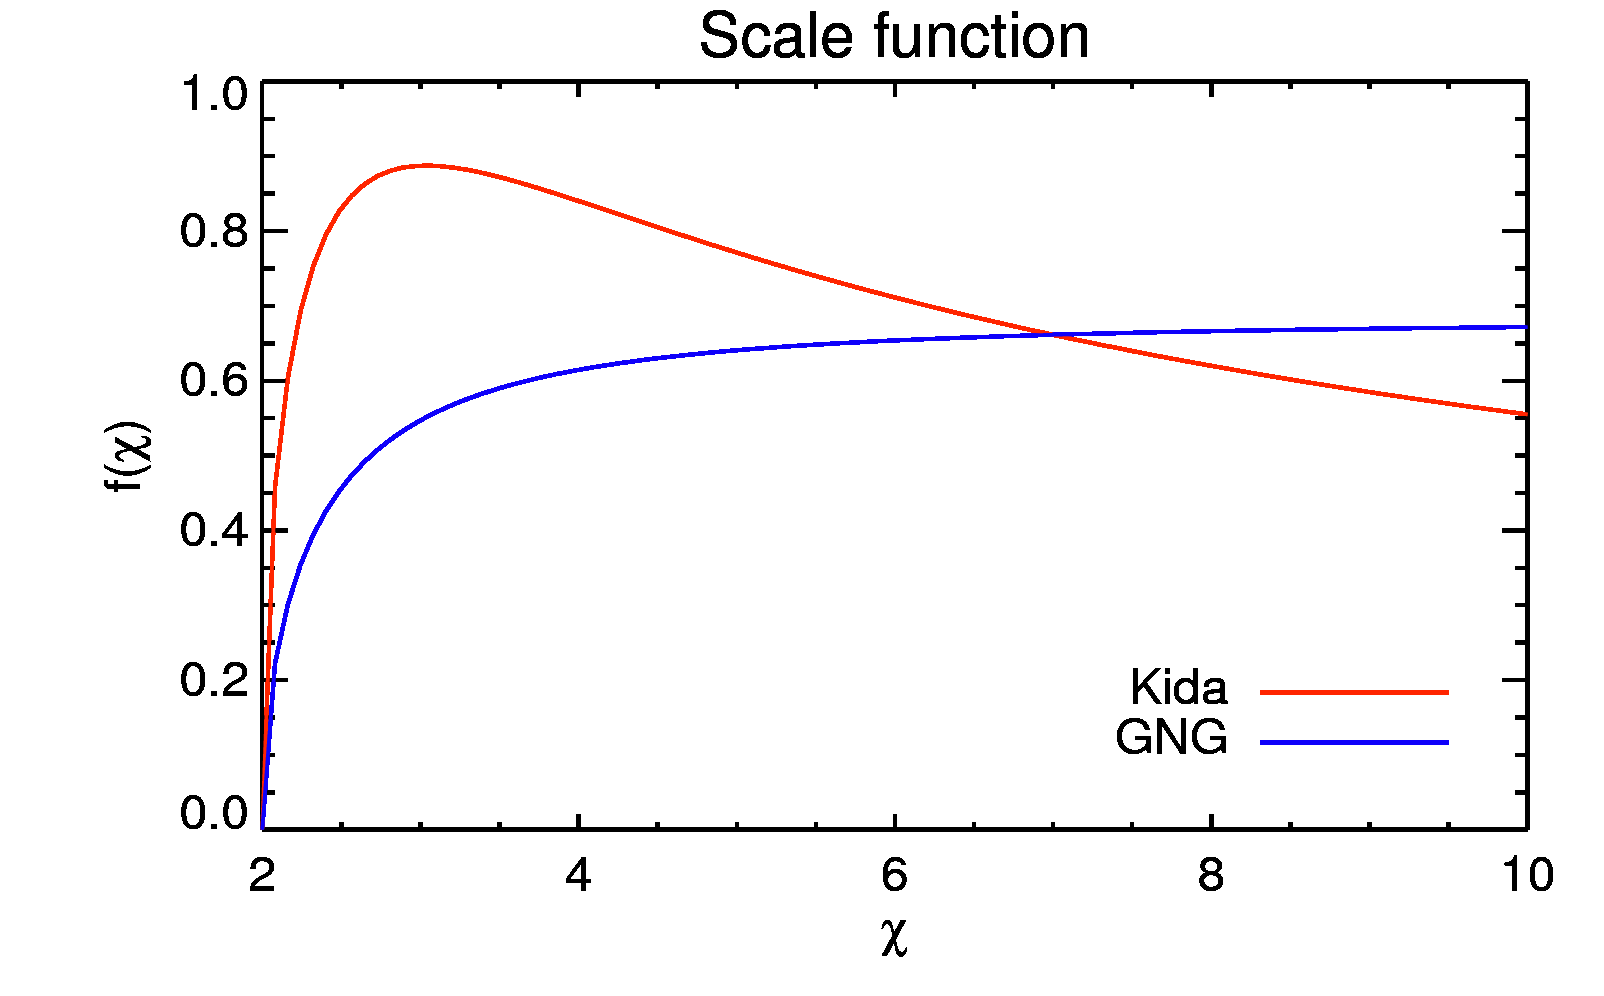
\includegraphics{../figs/scale_function.png}}
  \end{center}
\caption[]{The scale function $f(\chi)$, defined by
  \eq{eq:scale-function}, for the Kida ($\varOmega_V=3/2
  \ \varOmega_K/(\chi-1)$) and GNG ($\varOmega_V=\varOmega_K
  \sqrt{3/(\chi^2-1)}$ solutions, respectively. The scale function is
  related to the square root of the negative of the divergence
  \eqp{eq:scale-div}, and defined only for $\chi>2$. For smaller $\chi$ the
  divergence flips positive, meaning that dust is expelled from the
  vortex instead of getting trapped. This happens because of the
  correlation between $\varOmega_V$ and $\chi$. The aspect ratio shrinks
  as the vortex intensifies. At some point, the vortex rotates too
  fast, and particles are expelled by the centrifugal force (see e.g.,
  Chavanis 2000).}
 \label{fig:scale-function}
\end{figure}


\beq
\rho_d(a) = \rho_{d0} \ \exp\left(-\frac{a^2}{2H_V^2}\right) \ ,
\label{eq:gen_axi}
\eeq

\beq
 H_V = \frac{H}{f(\chi)} \sqrt{\frac{\delta}{\rm St}}. 
\label{eq:hv}
\eeq

The above solution is remarkable. Given the sonic scale $H$ and a vortex 
aspect ratio $\chi$, a single parameter ($\delta/{\rm St}$) controls the 
distribution of dust. This had already been 
hinted upon by Cuzzi et al. (1993) and Dubrulle et al. (1995) 
in the context of steady states of dust sedimentation. An insightful study by 
Jacquet et al. (2012) emphasized the relevance of this parameter for 
global redistribution of solids. Birstiel et al. (2013) also find this to be 
the parameter of relevance in their semi-analytical model. Dust distributions 
for different values of $\delta/{\rm St}$ are plotted in \fig{fig:gaussian}, as a 
function of $a/H$. We show in \fig{fig:disk}, in the inertial frame, 
the dust distribution for $\delta/St$=1 in a Kida vortex of $\chi=4$ embedded in a 
disk of aspect ratio is $H/r$=0.1. 

\begin{figure}
  \begin{center}
    \resizebox{\columnwidth}{!}{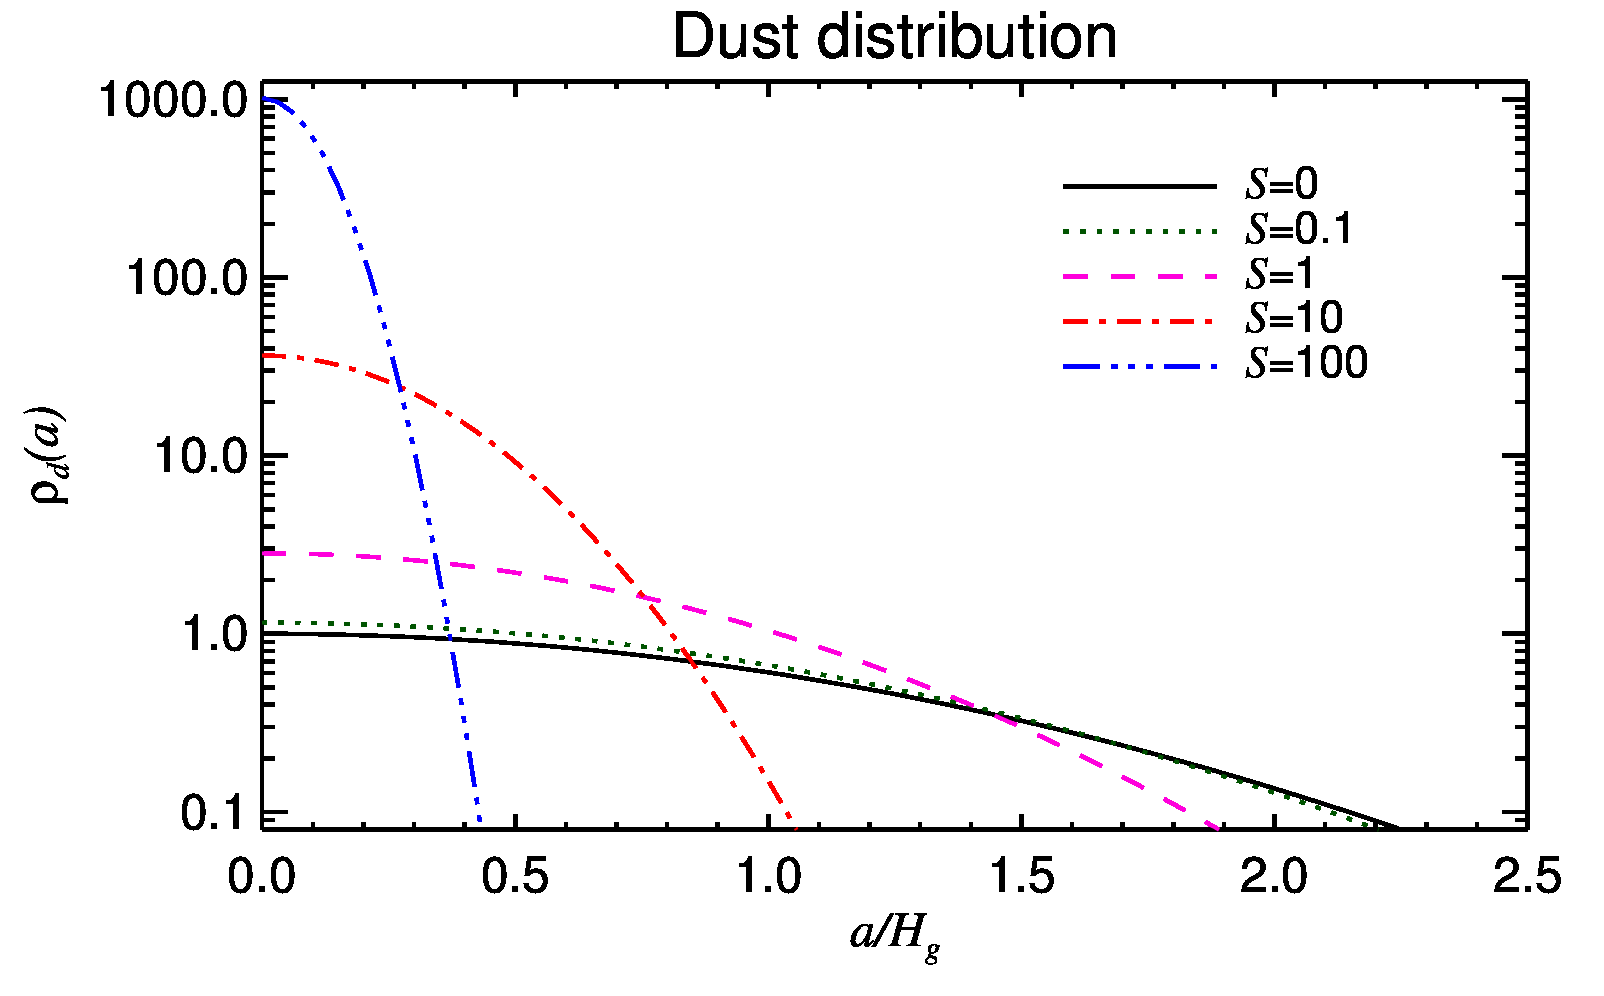
\includegraphics{../figs/gaussian.png}}
  \end{center}
\caption[]{Dust distribution for the axisymmetric case. As in
  \fig{fig:scale-function}, red and blue lines are for the Kida and
  GNG solutions, respectively. Distributions for $\delta/{\rm St}$=0.1, 1, and
  10 are shown (dashed, solid, and dot-dashed lines). The $x$-axis is
  $a/H$, where $H$ is the gas scale height. There is degeneracy
  between $\delta/{\rm St}$ and $f(\chi)$, as is clear from \eq{eq:hv}.}
 \label{fig:gaussian}
\end{figure}

\begin{figure}
\begin{center}
  \resizebox{\columnwidth}{!}{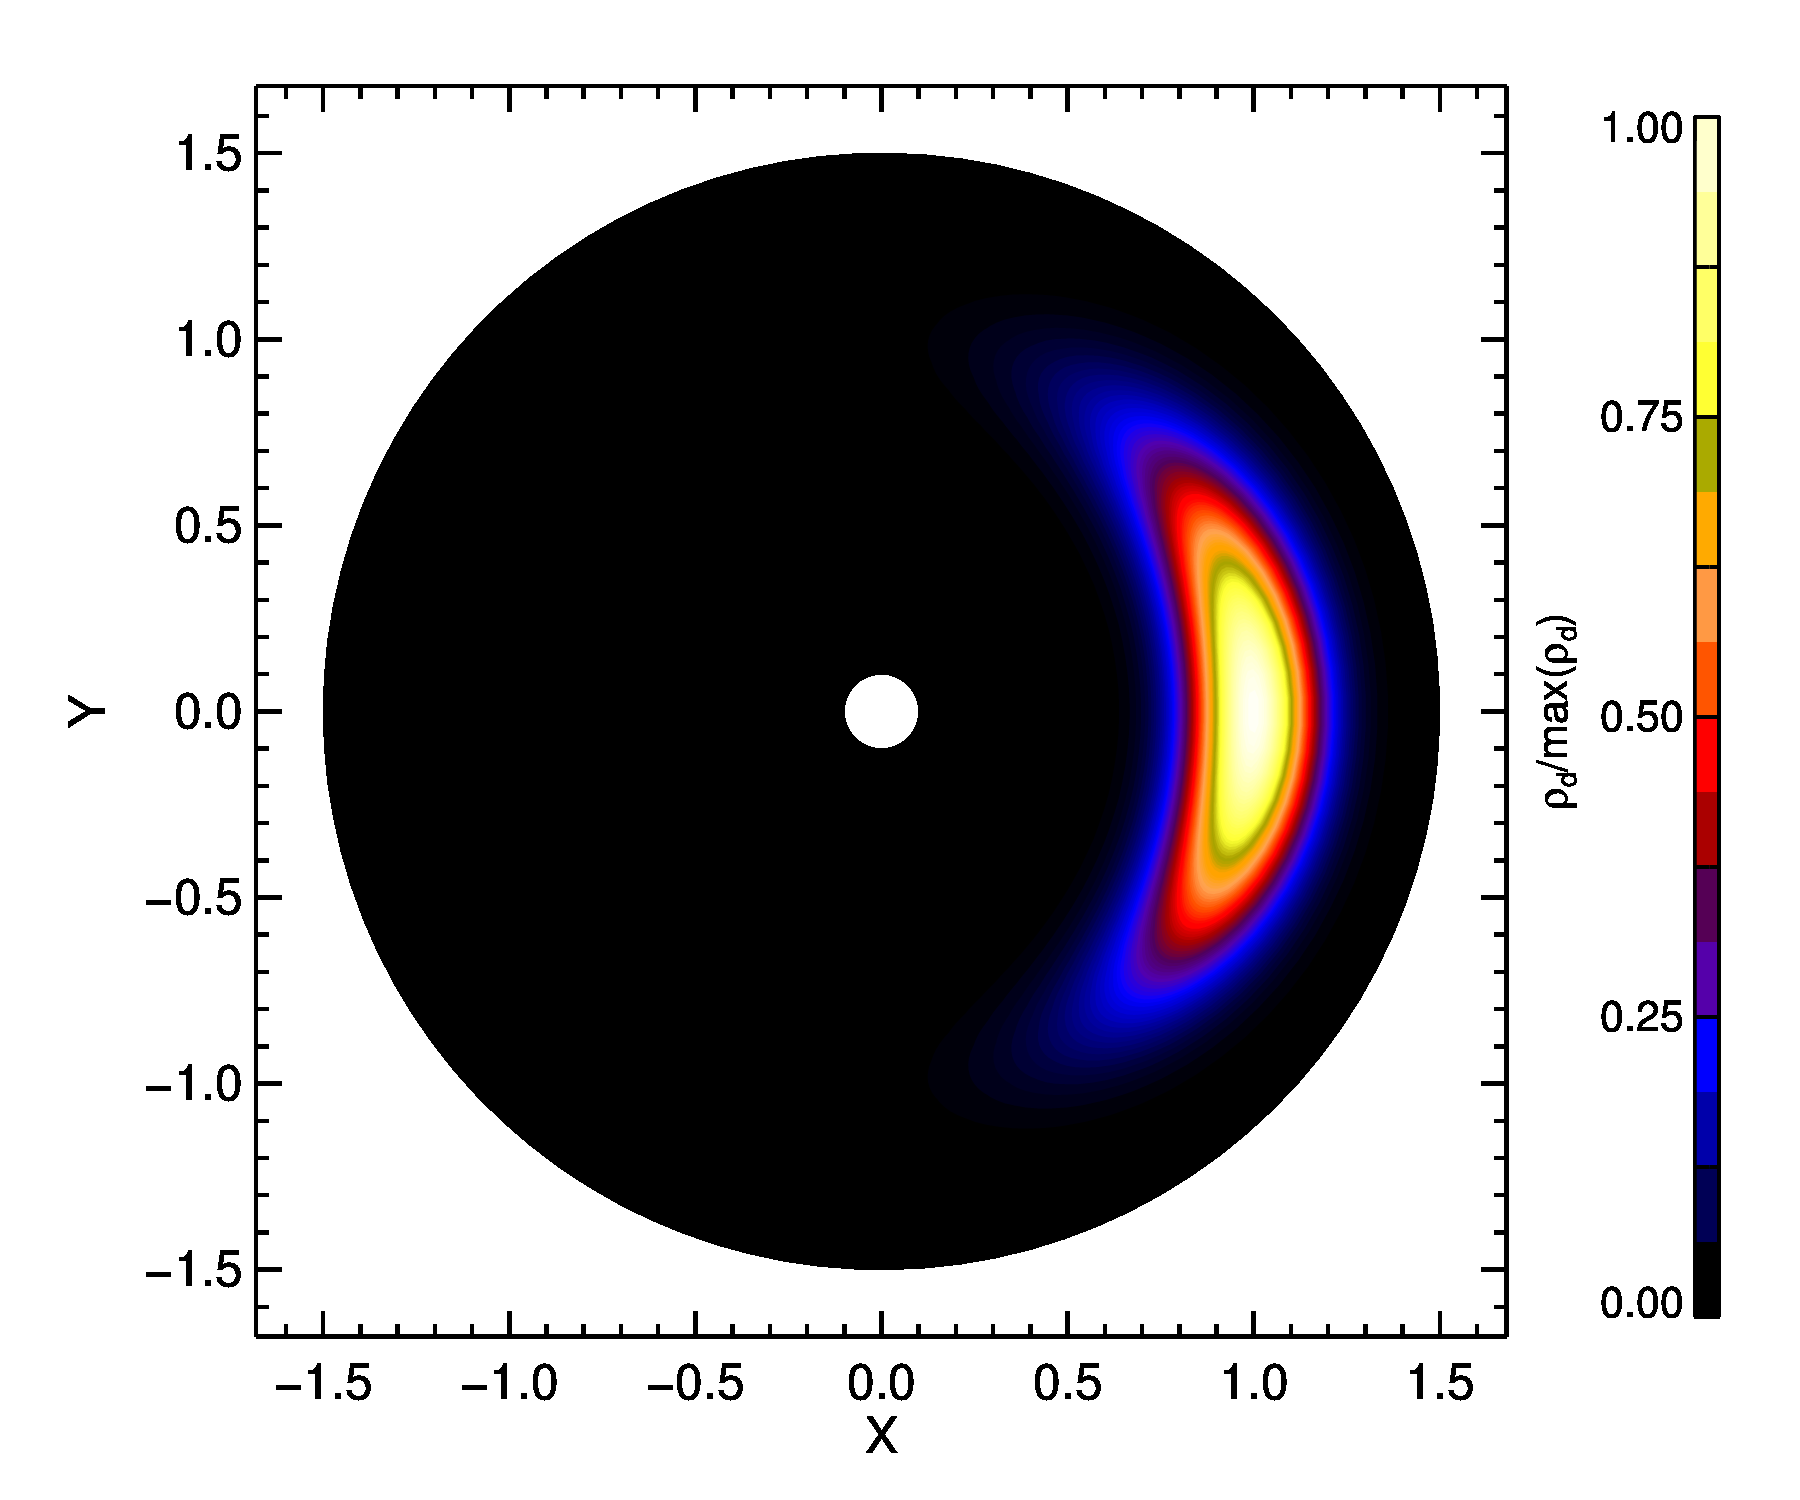
\includegraphics{../figs/disk.png}}
 \end{center}
\caption[]{Three parameters, plus a vortex solution, control the dust distribution. 
The figure shows the appearance of the dust trapped in a Kida vortex of $\chi=4$, 
for $\delta/St$=1, in a disk of aspect ratio $H/r$=0.1.}
 \label{fig:disk}
\end{figure}

\subsection{Axisymmetric $\v{u} = \v{v}$ }

It is illustrative to consider the case in which $|\v{u}| \gg \tau|\grad{h}|$,
so that we can approximate $\v{v}=\v{u}$ in the advection term.  In 
this case, \eq{eq:dust-trapping-uvzero} reduces to a relatively simple equation

\beq\label{eq:uveq}
\left(\Laplace{} + A\partial_\nu + B \right)\rho_d = 0. 
\eeq
%\eq{eq:uveq} compares dust diffusion to dust advection due to the
%vortex flow alone. 
\eq{eq:uveq} reflects dust diffusion (first term), dust advection due
to the vortex flow (second term) and dust concentration (third term). 
Note that we are effectively considering regions close to the vortex
center because $\nabla h$ vanishes there, while  
$\nabla^2h$ (i.e. $B$), does not.  

Now, assuming axis-symmetry and integrating in
$\frac{1}{2\pi} \int_0^{2\pi} d\nu$, we get  

\beq
\frac{\epsp}{2}\pderivn{\rho_d}{a}{2} +
\frac{\epsp}{2a}\pderiv{\rho_d}{a} + B \rho_d = 0.
\eeq

\noindent That is, 

\beq
y^{\prime\prime} + \frac{1}{a}y^\prime + k^2 y = 0, 
\label{eq:axisymmetric}
\eeq where $y(a) = \rho_d$ and $k$ is given by \eq{eq:k}. This
equation only differs from \eq{eq:dust-trapping-axis} through the
absence of the $k^2a\partial_a$ term, which occurs when the full
expression for the dust velocity is used. Clearly it is negligible 
for sufficiently small $a$. The general solution of \eq{eq:axisymmetric} is a
sum of Bessel functions of the first and second kinds: 

\beq
y(a) = c_1 J_0 (ka) + c_2 Y_0(ka). 
\eeq

\noindent Since  $Y_0$ diverges at the origin, we can physically discard 
this solution, setting $c_2=0$. So, the axisymmetric mode is $\rho(a)
= c_1 \ J_0 (ka)$, or

\beq
\rho(a) = c_1 \ J_0 \left(\frac{a}{H} \ f(\chi) \sqrt{\frac{2{\rm St}}{\delta}}\right).
\eeq 

The Bessel function $J_0(x)$ is
non-motononic, with the first root around $x=2.5$. The first zero is therefore around
$a_0 \approx H \sqrt{\delta/{\rm St}}$.  As the density
cannot be negative, that sets the validity of our solution. 
The solution is also constrained by our use of the shearing sheet
equations, so the results should not be valid for $x \gg H$.
As we made use of the approximation $\v{v}=\v{u}$, ${\rm St} \ll 1$,
and the solution  is indeed $a_0 \gg H$, for finite values of $\delta$.

We compare in \fig{fig:bessel-gaussian} the Bessel function with the exponential found in the
previous section for the general solution. They agree up to 10\% inside
$ka$=1.5 (i.e., $a/H_V\approx 1$), and up to 1\% within $ka$=1 (i.e., $a/H_V\approx 0.7$). Confident that the approximate
$\v{u}=\v{v}$ solution works well within the vortex core, we use this
approximation to find solutions to the full non-axisymmetric problem,
in the next section. 

\begin{figure}
  \begin{center}
    \resizebox{\columnwidth}{!}{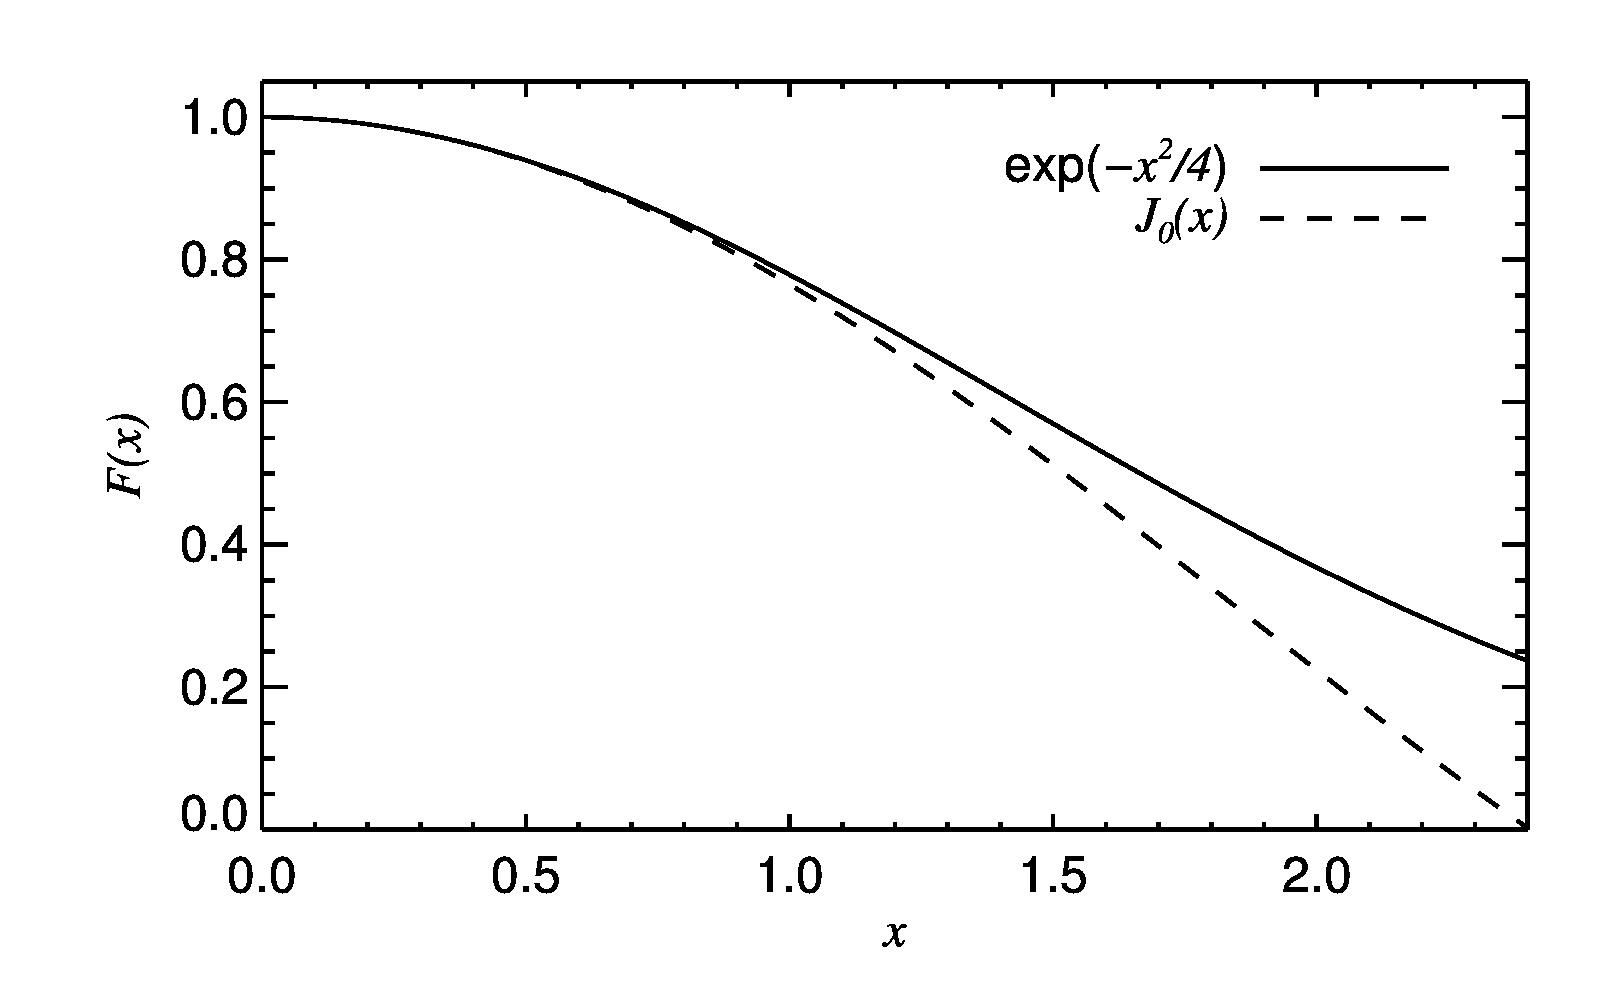
\includegraphics{../figs/bessel-gaussian.png}}
  \end{center}
\caption[]{The axisymmetric solutions for (solid line) the general 
$\v{v}=\v{u}+\tau\grad{h}$ case and, (dashed line) the case where
  we set $\v{v}=\v{u}$ for dust advection.
The exponential and Bessel solutions agree up to 10\% up to $x$=1.5, and up 
to 1\% up to $x$=1. We conclude that the latter approximate solution is quite accurate 
for describing the dust distribution in the vortex core.}
 \label{fig:bessel-gaussian}
\end{figure}


\section{Non-axisymmetric corrections}
We consider the non-axisymmetric problem ($\partial_\nu\neq0$) inside
the vortex core in the limit $\rm{St}\ll 1$. We formally set
$\bm{v}=\bm{u}$ in the advection term $\bm{v}\cdot\del$. Our
dust-trapping equation, \eq{eq:uveq}, then concerns advection due to 
the vortex flow alone. Physically, we expect that
including the $\tau$ term for dust velocity in the advection term only
helps to concentrate dust toward the vortex core (pressure maximum).      

\subsection{Conversion to ordinary differential equations}
The dust density $\rho_d$ is periodic in the $\nu$ co-ordinate. We
therefore seek solutions of the form

\beq\label{eq:series}
\rho_d(a,\nu) = {\rm Re}
\left[\sum_{n=0}^\infty\rho_n(a)\exp{\left(\mathrm{i}n\nu\right)} \right].
\eeq
For convenience, we will drop the real part notation from now on. Inserting
\eq{eq:series} into the partial differential equation \eqp{eq:dust-trapping-uvzero},
multiplying by $\exp{(-\mathrm{i}m\phi)}$, and integrating the resulting
expressions over the $\nu$ co-ordinate, we arrive at a set of 
ordinary differential equations, 
%\beqn\label{eq:ode1}
%&&0=\epsilon_{-}\left[\frac{1}{4}\rho_{m-2}^{\prime\prime}
%-\frac{1}{2a}\left(m-\frac{3}{2}\right)\rho_{m-2}^\prime +
%\frac{m(m-2)}{4a^2}\rho_{m-2}\right] \nonumber\\
%&&+\frac{\epsilon_+}{2}\left(\rho_m^{\prime\prime}+\frac{1}{a}\rho_m^\prime\right)
%-\left(\frac{m^2\epsilon_+}{2a^2}-\mathrm{i}mA-B\right)\rho_m\nonumber\\
%&&+\epsilon_{-}\left[\frac{1}{4}\rho_{m+2}^{\prime\prime}
%+\frac{1}{2a}\left(m+\frac{3}{2}\right)\rho_{m+2}^\prime +
%\frac{m(m+2)}{4a^2}\rho_{m+2} \right]
%\eeqn
%for each $m$. We only consider even $m$ \comm{why?}. For $m=0$, the $\rho_{m-2}$
%terms are absent. We require $\rho_m^\prime(0)=0$ and
%$\rho_{m\geq2}(0)=0$ \comm{why?}. 
%It will be convenient to write the above equations
%in operator form,

\beq\label{eq:ode2}
\tilde{\chi}\mathcal{B}_m\rho_{m-2}(z) + \mathcal{A}_m\rho_m(z) + \tilde{\chi}\mathcal{C}_m\rho_{m+2}(z)=0,
\eeq
where $z\equiv ka$, $\tilde{\chi}\equiv(\chi^2-1)/[2(\chi^2+1)]$, and 
\beqn\label{eq:ops}
\mathcal{B}_m &\equiv& \frac{d^2}{dz^2} -
\frac{2}{z}\left(m-\frac{3}{2}\right)\frac{d}{dz} + \frac{m(m-2)}{z^2},\\
\mathcal{A}_m &\equiv& \frac{d^2}{dz^2} + \frac{1}{z}\frac{d}{dz} +
\left(k_m^2 - \frac{m^2}{z^2}\right),\\
\mathcal{C}_m  &\equiv& \frac{d^2}{dz^2} +
\frac{2}{z}\left(m+\frac{3}{2}\right)\frac{d}{dz} +
\frac{m(m+2)}{z^2}, 
\eeqn
where $k_m^2 \equiv 1+\mathrm{i}mA/B$. \eq{eq:ode2} holds for each
$m$ except for $m=0$ for which the $\rho_{m-2}$ terms are absent. Each
$\rho_m$ couples to $\rho_{m\pm2}$ through operators $\mathcal{B}_m$
and $\mathcal{C}_m$. The axisymmetric problem is recovered by
setting $\rho_{m>0}=0$. (We remark that a similar set of ODEs may be
derived when the full expression for dust velocity is used.)  
%The coupling terms vanish for $\chi=1$, as
%expected, since in that case the vortex flow is truly axisymmetric.    

In the limit $\rm{St}\ll 1$, dust is advected by fluid with elliptic
streamlines, so we expect $\rho_d(a,\nu)$ to have even symmetry in
$\nu$. Henceforth we only consider even $m$. We seek solutions with  
$\rho_m^\prime(0)=0$ and $\rho_{m\geq2}(0)=0$, so that
$\partial_x\rho_d=\partial_y\rho_d=0$ at the origin, consistent with 
dust reaching maximal density there.  

%It will be convenient to write the above equations
%in operator form,
Finally, we note that
\beqn\label{eq:ops2}
\mathcal{B}_mJ_{m-2}(\mu z) &=& \mu^2J_m(\mu z),\\
\mathcal{A}_mJ_m(\mu z) &=& \left(k_m^2 - \mu^2\right)J_m(\mu z),\\
\mathcal{C}_mJ_{m+2}(\mu z) &= & \mu^2J_m(\mu z),
\eeqn
where $\mu$ is a constant. These relations will be useful in
constructing solutions. 

\subsection{$z\ll 1$}
For small $\rm{St}$, $z=ka$ is small. As $z\to 0$, we expect $\rho_0$
becomes the dominant term in \eq{eq:series} because the
non-axisymmetric components vanish at the origin. Furthermore, we
require $|\rho_m|$ to decrease with respect to $m$ in order to achieve
convergence. This motivates us to seek the simplest non-axisymmetric solution as  
\beq
\rho_d(z,\nu) \simeq \rho_0(z) + \rho_2(z)\exp{\left(2\mathrm{i}\nu\right)},  
\eeq
for $z\ll 1$. We proceed as follows. Let
\beq
\rho_0(z) = D_0J_0(k_0z) + \epsilon(z),  
\eeq
where $\epsilon(x)$ represents the correction to the axisymmetric
solution due to $\rho_2(z)$. $D_0$ is a constant not to be confused
with diffusion. The ODEs to be
solved are 
\beqn 
\mathcal{A}_0\epsilon(z) &=& -\tilde{\chi}\mathcal{C}_0\rho_2(z),\label{eq:m2_eq1}\\
\mathcal{A}_2\rho_2(z) &=& -\tilde{\chi}\left[D_0k_0^2J_2(k_0z) +
  \mathcal{B}_2\epsilon(z)\right].\label{eq:m2_eq2} 
\eeqn

To make further progress, at this stage we \emph{assume} that the
$\epsilon$ term in \eq{eq:m2_eq2} can be neglected. Thus $\rho_2$ satisfies
\beq\label{eq:rho2_approx}
\mathcal{A}_2\rho_2(z) \simeq -\tilde{\chi}D_0k_0^2J_2(k_0z).
\eeq
This can be solved by 
\beq\label{eq:rho2_approx_sol}
\rho_2(z)  = -\frac{\tilde{\chi}D_0k_0^2J_2(k_0z)}{k_2^2 - k_0^2}, 
\eeq
implying the axisymmetric solution from the previous section, 
$J_0(z)$, acts as a source for the $m=2$ non-axisymmetric
component. Note that because we are considering $\rm{St}\ll1$ and
therefore $|k_2^2|\gg1$, Eq. \ref{eq:rho2_approx_sol} indicates $\rho_2$
is a small perturbation to the axisymmetric solution.     


%The general solution to \eq{eq:rho2_approx} includes the
%complementary function $J_2(k_2z)$. However, $k_2$ is complex and
%$|k_2|\gg 1$ (because we are considering $\mathrm{St}\ll1$), so $J_2(k_2z)$
%may not be well behaved at boundaries. To avoid complications from
%Bessel functions of complex arguments, we have therefore taken the
%particular integral to \eq{eq:rho2_approx} as the solution for
%$\rho_2$. This is to regard $\rho_0$ as a source term for
%$\rho_2$ . For $|k_2^2|\gg 1$, Eq. \ref{eq:rho2_approx_sol} indicates  
 
We can use \eq{eq:rho2_approx_sol} in \eq{eq:m2_eq1} to
calculate the correction term $\epsilon$. We find 
%The ODE to solve is
%\beqn
%\mathcal{A}_0\epsilon(x)
%&=&\frac{\tilde{\chi}^2D_0k_0^2}{k_2^2-k_0^2}\mathcal{C}_0J_2(k_0x) \nonumber \\ 
%&=&\frac{\tilde{\chi}^2D_0k_0^4J_0(k_0x)}{k_2^2-k_0^2}.
%\eeqn
%The particular integral is 
\beq
\epsilon(x) = \frac{\tilde{\chi}^2D_0k_0^3xJ_1(k_0x)}{2\left(k_2^2 -
  k_0^2\right)}. 
\eeq
This term is also small because of $|k_2^2|\gg1$. Furthermore, it is
smaller than $\rho_2(z)$ by a factor $\tilde{\chi}$.  

We plot $|\rho_2|/|\rho_0|$ as a function of $z$ in \fig{fig:nonaxi}, 
for $\chi=10$ and $\rm{St}=0.3$. We see that for $z\lesssim 1$, even 
for such a not-so-small Stokes number, the deviations from axisymmetry
is on the order a few per cent. This is attributed to the fact
that the corrections involve higher order Bessel functions, which
becomes small compared to $J_0$ for small $z$.   

Collecting the above results and Taylor-expanding the Bessel functions, our
weakly non-axisymmetric solution for $z\ll 1$ reads:

%\beqn
%\rho_0(z) &=& D_0\left[1 -
%  \frac{k_0^2z^2}{4}\left(1-\frac{\tilde{\chi}^2k_0^3}{k_2^2-k_0^2}\right)
%+ O(z^4)\right],\\
%\rho_2(z) &=&
%-\frac{D_0\tilde{\chi}k_0^2}{(k_2^2-k_0^2)}\left[\frac{k_0^2z^2}{8}+O(z^4)\right].  
%\eeqn 

\beqn
\rho_0(z) &=& D_0\left[1 -
  \frac{z^2}{4}\left(1-\frac{\tilde{\chi}^2B}{2\mathrm{i}A}\right)
+ O(z^4)\right],\\
\rho_2(z) &=&
-\frac{D_0\tilde{\chi}B}{2\mathrm{i}A}\left[\frac{z^2}{8}+O(z^4)\right],  
\eeqn 
where we used the definition of $k_m$. 

In the previous section, we obtained the axisymmetric solution
assuming the axisymmetric components are negligible. Here, we 
see explicitly that the axisymmetric solution in fact leads to
non-axisymmetry through the coupling terms, but these corrections are
small for $\rm{St}\ll1$, because $B\propto\mathrm{St}$. 
We conclude that dust in the vortex core is effectively axisymmetric.   

\begin{figure}
  \begin{center}
    \resizebox{\columnwidth}{!}{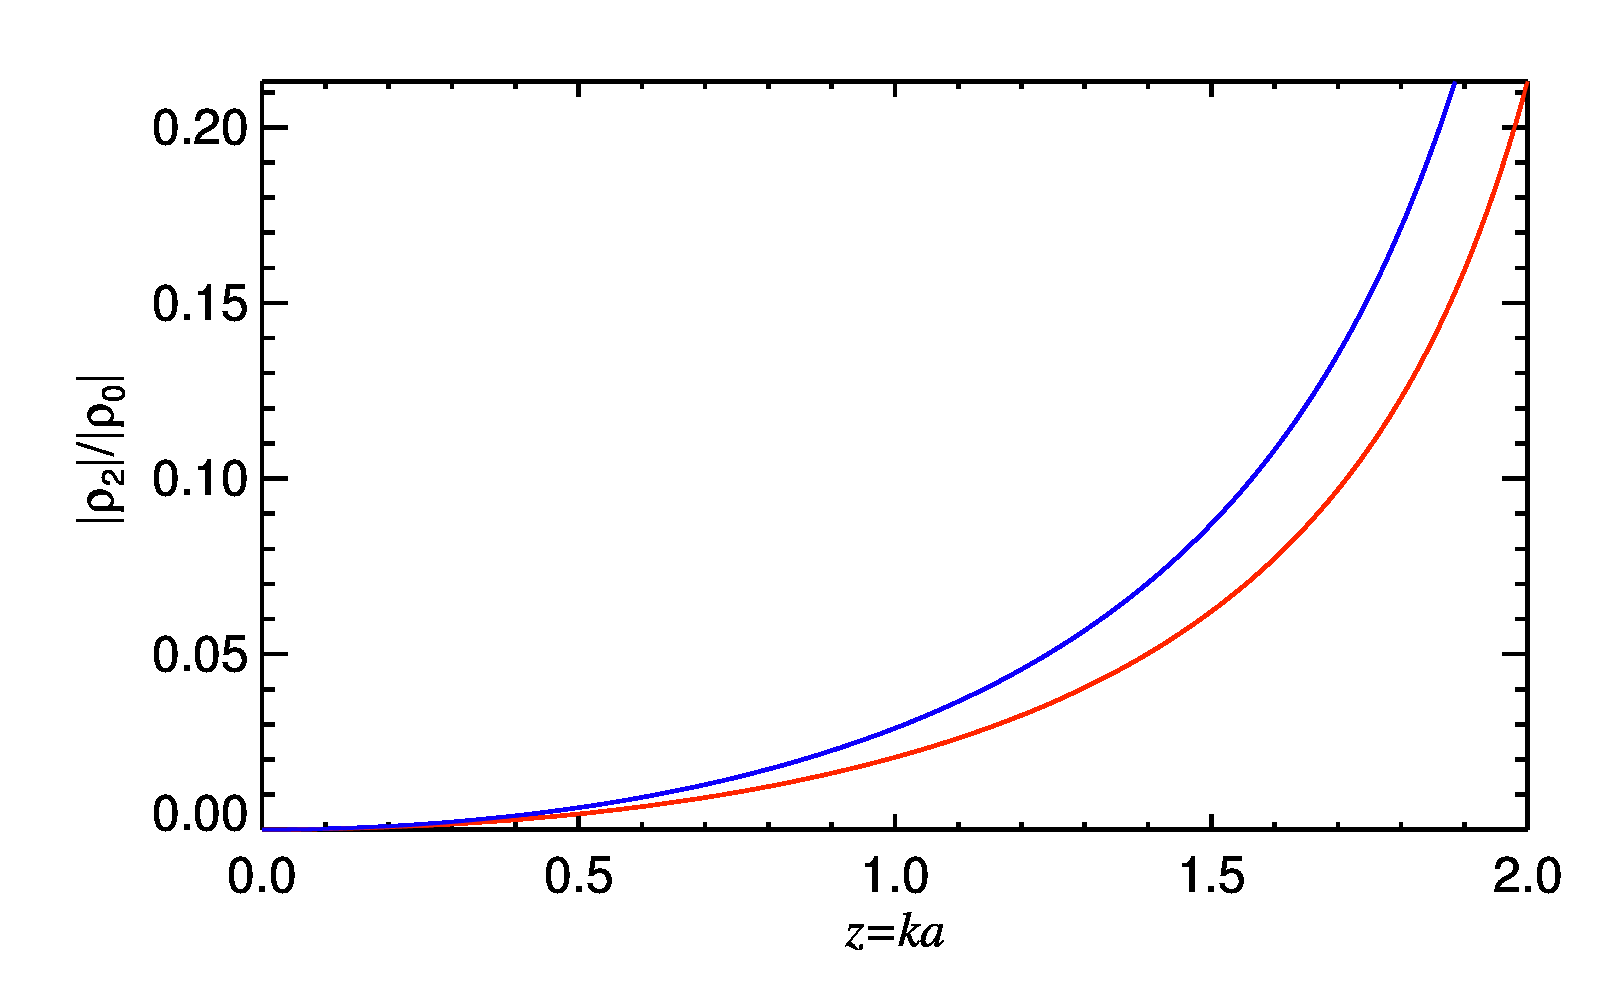
\includegraphics{../figs/nonaxi.png}}
  \end{center}
  \caption[]{Magnitude of the $m=2$ non-axisymmetric component normalized by the magnitude of the axisymmetric part of the solution, for the Kida vortex (red) and GNG vortex (blue) of aspect-ratio $\chi=10$ and Stokes number $\rm{St}=0.3$. }
 \label{fig:nonaxi}
\end{figure}



\subsubsection{Consistency check}
Using the above expression for $\epsilon(x)$, we can evaluate
$\mathcal{B}_2\epsilon(x)$ in order to assess our assumption that
$\epsilon(x)$ has a negligible contribution to $\rho_2$. We find
\beq
\mathcal{B}_2\epsilon(z) =
-\frac{\tilde{\chi}^2D_0k_0^5zJ_1(k_0z)}{2\left(k_2^2 -
  k_0^2\right)}. 
\eeq
Provided that $|k_2^2|\gg1$, this term is indeed small compared to the
first term on the RHS of Eq. \ref{eq:m2_eq2}. Furthermore, because
$zJ_1(z)\propto z^2$ for $z\ll1$, this term causes a small correction
to $\rho_2$ at $O(z^4)$ via Eq. \ref{eq:m2_eq2}. Our solution 
procedure above is self-consistent.  

%Both the $\tilde{\chi}^2$ term and the $k_2^2$ term contributes to
%making $\mathcal{B}_2\epsilon$ small in comparison to the $J_2$ term
%on the RHS of \eq{eq:m2_eq2}. 
%An iteration scheme can now be set up. One can update
%$\rho_2$ with the inclusion of $\mathcal{B}_2\epsilon(x)$ using
%\eq{eq:m2_eq2}, then in turn update $\epsilon(x)$ using
%\eq{eq:m2_eq1} and so on. 

\subsection{Lower $m$ mode as a source for higher $m$ mode}
We can extend the above procedure to obtain approximate solutions for
$\rho_{m>2}$. We regard $\rho_{m-2}$ acts as a source for $\rho_{m}$. That is
\beq\label{eq:higherm}
\mathcal{A}_m\rho_m(x) = -\tilde{\chi}\mathcal{B}_m\rho_{m-2}. 
\eeq 
Then, by induction,
\beq\label{eq:induction}
\rho_m(x) =D_0
\frac{(-1)^{m/2}\tilde{\chi}^{m/2}k_0^m}{\prod_{l=1}^{m/2}(k_{2l}^2-k_0^2)}J_m(k_0x). 
\eeq
Although Eq. \ref{eq:higherm} is artificial, the closed-formed
approximate solutions, Eq. \ref{eq:induction}, may be useful as initial
guesses for a numerical relaxation scheme. It also explicitly shows that the
magnitudes of the induced higher $m$ modes decay with $m$.  

%\begin{figure}
%\begin{center}
%  \resizebox{\columnwidth}{!}{\includegraphics{../figs/gaussian-bessel.png}}
% \end{center}
%\caption[]{.}
% \label{fig:gaussian-bessel}
%\end{figure}


\section{Conclusions}

\acknowledgments

\begin{thebibliography}{}
\expandafter\ifx\csname natexlab\endcsname\relax\def\natexlab#1{#1}\fi

\bibitem[{{Calvet et al.}(2005)}]{Calvet05} Calvet, N., D'Alessio, P.,
  Watson, D. M., Franco-Hernández, R., Furlan, E., Green, J., Sutter,
  P. M., Forrest, W. J., Hartmann, L., Uchida, K. I., Keller, L. D.,
  Sargent, B., Najita, J., Herter, T. L., Barry, D. J., \& Hall,
  P. 2005, ApJ, 630, 185



\end{thebibliography}

\end{document}
